% ======================================================================


% Sujet du document
% Informations importantes
%
%
% Prénom Nom
% H. Dube 2019
% ======================================================================
% Ce code rassemble les efforts d'étudiants de la faculté de génie  
% de l'université de Sherbrooke afin de faire un template LaTeX moderne
% dédié à l'écriture de rapport universitaire.
% Ce document est libre d'être utilisé et modifié.
% ======================================================================

% ----------------------------------------------------
% Initialisation
% ----------------------------------------------------
\documentclass{udes_rapport} % Voir udes_rapport.cls

\begin{document}
\selectlanguage{french}

% ----------------------------------------------------
% Configurer la page titre
% ----------------------------------------------------

% Information
\faculte{Génie}
\departement{génie électrique et génie informatique}
\app{5}{Conception d’asservissements analogiques}
\professeur{Karina Lebel}
\etudiants{Hubert Dubé - dubh3401 \\ Gabriel Lavoie - lavg2007}
\dateRemise{15 novembre 2019}


% ======================================================================
\pagenumbering{roman} % met les numéros de pages en romain
% ----------------------------------------------------
% Page titre
% ----------------------------------------------------
\fairePageTitre{LOGO} % Options: [STD, LOGO]
\newpage

% ----------------------------------------------------
% Table des matières
% ----------------------------------------------------
\tableofcontents
\newpage


% ----------------------------------------------------
% Table des figures
% ----------------------------------------------------
\listoffigures
\newpage

% ----------------------------------------------------
% Table des tables
% ----------------------------------------------------
\listoftables
\newpage



% ======================================================================
% Document
% ======================================================================
\pagenumbering{arabic} % met des chiffres arabes
\setcounter{page}{1} % reset les numéros de pages
%%%%%%%%%%%%%%%%%%%%%%%%%%%%%%%%%%%%%%%%%%%%%%%%%%%%%%
%{Analyse du signal
%%%%%%%%%%%%%%%%%%%%%%%%%%%%%%%%%%%%%%%%%%%%%%%%%%%%%%
\section{Introduction}
\section{Procédure de conception systématique}
%----------------------------------------------------------------------------------------------------------------------%
\section{Design du télescope A}
\subsection{Azimut}
Avant de commencer le desing de compensateur, posons un regard sur le la réponse à l'échellon et sur le lieu de bode de la fonction de transfert qui sera à l'étude dans la prochaine partie.\\
%%%%%%% FIGURE %%%%%%%
%double figure
\makebox[\textwidth][c]{
\noindent\begin{minipage}{1.3\textwidth}
 
\begin{minipage}{0.5\textwidth}
\insertFigure{double}{FTBO_AZ}{1}{Réponse à l'échellon de l'azimut original}
\end{minipage}%
\begin{minipage}{0.5\textwidth}
\insertFigure{double}{marges_FTBO_AZ}{1}{Marges de l'azimut original}
\end{minipage} 

\captionof{figure}{Observation initial} 
\label{fig:init_A_AZ} 
\end{minipage}
}
%%%%%%%%%%%%%%%%%%%%%%
\subsubsection{Design initial}
Le début de la conception est de déterminer la position des pôles désirés. Ceux-ci représentes les emplacement par lesquels le lieu des racines devra passer afin de satisfaire les demandes de design du client. Cette partie est faite dans le document \textit{trad\_specs.m} . Les caractéristiques d'équations de système d'ordre 2 standards y sont déterminé, soit $\zeta$ et $\omega _{n}$. À partir du critère de dépassement maximal, $\zeta$ est calculé à $0.4037$. Il y a par contre plusieurs valeurs de $\omega _{n}$ possibles, ce qui demande de vérifier lequel sera le plus approprié au contexte présent. Dans notre cas, le $\omega _{n}$ de $11.1484$ est lui à choisir, car il est le plus grand, ce qui permettera l'atteinte de tous les autres critères de design (prendre le $\omega _{n}$ le plus grand assure de respecter tous les temps de monté). Ainsi, les pôles désirés sont:
\[s^* = -4.5008\pm 10.1995i\]
Ensuite , il est possible de déterminer le types de compensation désiré. En affichant la réponse à un échellon, il est clair que la réponse transitoire du système doit être amélioré. Pour ce faire, un compensateur par avance de phase doit être utilisé afin de réduire la réponse en haute fréquence qui correspond à la section transitoire. La technique de la bissectrice sera utilisée de la manière suivante:
Avancer la phase implique de stabiliser le système et donc de le tirer vers la droite sur le lieu des racines. Le calcul de $\Delta \phi$ permet de déterminer quel changement doit être appliqué à la phase pour la réduire à celle d'un système à phase minimale.
\[\Delta \phi = -180 - \langle G(s)\vert_{s = s^*} \rangle\]
\[\Delta \phi = 73.0918^\circ \]
Comme la phase à compenser est positive, il est évident qu'une compensation par avance de phase est à faire. Les valeurs du zéro et du pôle est ensuite déterminé à partir de ce changement à appliquer. Le gain à compenser est calculé en fonction du positionnement du zéro et du pôle sur l'axe réel et du gain de la fonction à compenser.
\[AvPh = k_a\frac{s-z}{s-p}\]
\[k_a = \frac{1}{AvPh \vert_{s = s^*} \cdot \vert G(s^*)  \vert } \]
\[AvPh_1 = 11.5353 \cdot \frac{s+3.8857}{s-31.9861}\]
Le résultat de l'avance de phase avec $AvPh_1$ est affiché à la  figure \ref{fig:FTBO_AZ_AvPh_marge} pour les marges et la réponse à un échellon unitaire à la figure \ref{fig:step_A_AZ_comp_wcb_no}.
%%%%%%% FIGURE %%%%%%%
\insertFigure{simple}{FTBO_AZ_AvPh_marge}{0.7}{Lieu de bode de l'azimut corrigé avec un AvPh}
%%%%%%%%%%%%%%%%%%%%%%
Un avance de phase a été utilisé afin de ne pas amplifier le bruit que pourrait engendrer un PD. En effet, le très grand gain causé par le PD sur les hautes fréquences viendrait nuire au respect de la demande du client de \textit{minimiser l’amplification du bruit des capteurs pour le Télescope A}. Il en sera de même pour la fonction de transfert en élévation, si une compensation en avance de phase est nécessaire.

\subsubsection{Design final}

L'ajout de ce dernier compensateur améliore le régime transitoire, mais ne permet pas de répondre aux spécifications de sécurité. Un autre compensateur d'avancement de phase est donc nécessaire pour respecter le marge de retard acceptable. Un approche par la méthode de bode doit être utilisé, car les spécifications sont dans le domaine fréquentiel. La marge de phase désirée est calculée à la fréquence de traverse en gain afin de déterminer par combien la phase du système doit être augmentée. Le gain permetant la traverse en fréquence doit rester le même parce que les caractéristiques $\zeta$ et $\omega _{n}$ doivent être conservés. Le $K^*$ est donc de 1.
La marge de phase nécessaire est 
\[ TM = \frac{PM^*}{\omega_n}\cdot\frac{\pi}{180}\]
\[PM^* = 52.8378^\circ\]
On obtient donc la phase à compenser
\[\Delta \phi = PM^* - PM \]
\[\Delta \phi = 20.6660^\circ\]
Où $PM$ est la marge de phase du système à corriger (système corrigé seulement par le premier AvPh). En utilisant les formules de la page 28 du chapitre 7 des notes de Jean de LaFontaine, le compensateur suivant est obtenu
\[AvPh = k_a\frac{s-z}{s-p}\]
\[k_a = \frac{K^*}{\vert \frac{s-z}{s-p} \vert}\]
\[ AvPh_2 =  1.3933 \cdot \frac{s+6.6186}{s+12.8493}\]
Où $k_a$ est le gain à appliquer au filtre pour enlever l'impacte qu'il aurait sur la fréquence de traverse en fréquence.

Comme il est possible de le voir sur la figure \ref{fig:step_A_AZ_comp_wcb_no}, il reste une bonne quantité de raisonnance dans le système en azimut après l'ajout de $  AvPh_2 $. Pour réduire, voir éliminer, ce phénomène, un filtre coupe bande est utilisé directement dans la boucle ouverte. La fréquence de coupure de celui-ci est déterminé par la fréquence du pic dans le lieu de bode () et une largeur de 12 rad par seconde est utilisée afin de minimiser l'impacte général du coupe bande sur le reste du système. Le coupe bande obtenu est donc :
\[H(s) = \frac{s^2 - 54.8^2}{s^2 + 12s + 54.8^2}\]
Et l'application de celui-ci résulte à la réponse à l'échellon de la figure\ref{fig:step_A_AZ_comp_wcb_no}.

%%%%%%% FIGURE %%%%%%%
%double figure
\makebox[\textwidth][c]{
\noindent\begin{minipage}{1.3\textwidth}
 
\begin{minipage}{0.5\textwidth}
\insertFigure{double}{step_A_AZ_comp_wcb_no}{1}{Comparaison des réponses à l'échellon}
\end{minipage}%
\begin{minipage}{0.5\textwidth}
\insertFigure{double}{marges_A_AZ_no}{1}{Marges à la suite de tous les compensateurs et le filtre}
\end{minipage} 

\captionof{figure}{Observation suite à l'ajout d'un second AvPh et d'un coupe-bande} 
\label{fig:mid_A_AZ} 
\end{minipage}
}
%%%%%%%%%%%%%%%%%%%%%%


La figure \ref{fig:step_A_AZ_comp_wcb} montre bien l'effet de l'ajout des compensateurs d'avance de phase et du coupe bande, mais les calculs de temps de monté, de dépassement maximal et de stabilisation montrent les défaults restants après toutes les corrections ajoutées précedemment. En effet, la marge de retard n'est pas plus grande que 0.1, comme la marge de phase de la figure \ref{fig:marges_A_AZ_no} le fait remarquer. Pour rectifier cette situation, il a suffit d'ajouter une petite surcompensation, trouvée par itération, initialement au $\Delta \phi$ du premier compensateur afin de prévenir le retard de phase créé par l'ajout du coupe bande. Une fois cette dernière modification faite, les résultats finaux sont obtenus et seront évalués dans la section \ref{valid_AZ_A}. Comme il y a beaucoup d'ajout de compensateur et de filtre entre les spécifications initiales et le résultat final, il est normal d'avoir à faire un ajustement itératif à la fin du processus de design. L'ajout de plusieurs filtres en cascade vient modifier légèrement les résultats obtenus précédemment et les calculs pour prédire chacun des changements prendrait beaucoup plus de temps que de seulement itérer sur quelques valeurs précises. Une fois les itérations faites, voici la fonction de transfert du deuxième compensateur d'avance de phase.
\[ AvPh_2 =  1.4459 \cdot \frac{s+6.3777}{s+13.3346}\]

%%%%%%% FIGURE %%%%%%%
%double figure
\makebox[\textwidth][c]{
\noindent\begin{minipage}{1.3\textwidth}
 
\begin{minipage}{0.5\textwidth}
\insertFigure{double}{step_A_AZ_comp_wcb}{1}{Comparaison des réponses à l'échellon finale en azimut}
\end{minipage}%
\begin{minipage}{0.5\textwidth}
\insertFigure{double}{marges_A_AZ}{1}{Marges à la suite du correctif de $\Delta \phi$}
\end{minipage} 

\captionof{figure}{Observation final} 
\label{fig:final_A_AZ} 
\end{minipage}
}
%%%%%%%%%%%%%%%%%%%%%%




\newpage
\subsubsection{Conformité}
\begin{center}
  \captionof{table}{Conformité de l'azimut du télescope A}
  \label{tab:conformite_A_AZ}
  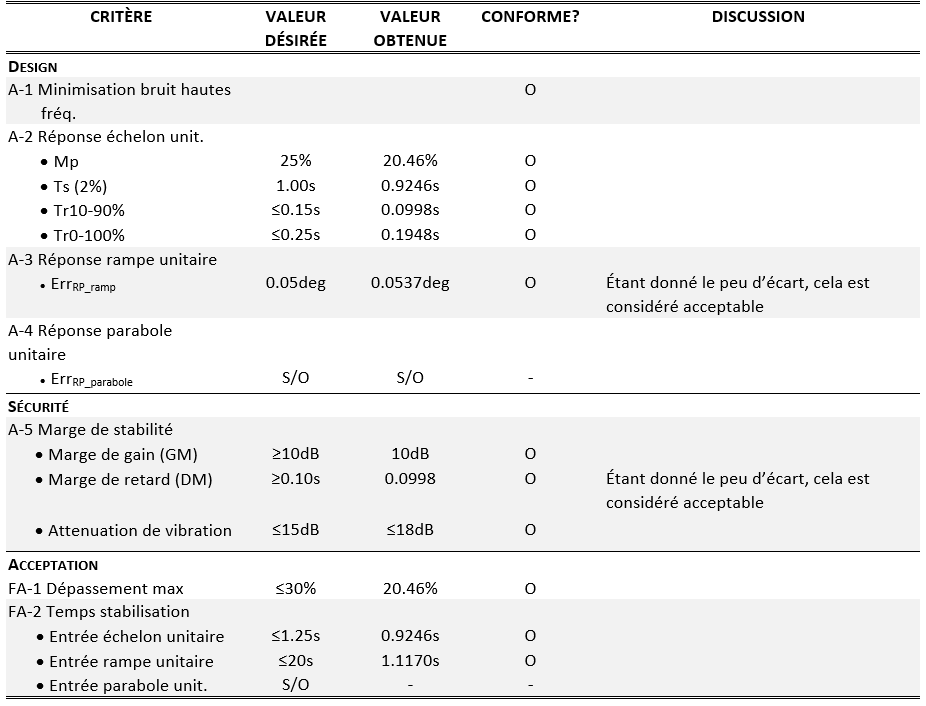
\includegraphics[width=\linewidth]{conformite_A_AZ}
\end{center}

Le tableau \ref{tab:conformite_A_AZ} présentes les différents critères du clients et les caractéristiques rencontrés par le système de compensation développé plus haut. La majorité des spécificaitons sont rencontrées.\\
La minimisation de l'amplification des hautes fréquences est évaluer de manière qualitative à l'aide de la figure \ref{fig:HF_minimal_AZ}. Comme il est possible de le voir, il n'y a que très peu de gain appliqué entre la finale et l'originale dans les hautes fréquence. Deplus, l'orde du gain de cette zone est plus petit que -100 dB, il est donc possible de considérer que les hautes fréquences (le bruit) a été augmenté de manière minimale. Sur l'agrandissement \ref{fig:HF_minimal_AZ_zoom} il est mis en évidence que le gain des vibrations est inférieure à -15dB.
%%%%%%% FIGURE %%%%%%%
%double figure
\makebox[\textwidth][c]{
\noindent\begin{minipage}{1.3\textwidth}
 
\begin{minipage}{0.5\textwidth}
\insertFigure{double}{HF_minimal_AZ}{1}{Comparaison des lieux de bode}
\end{minipage}%
\begin{minipage}{0.5\textwidth}
\insertFigure{double}{HF_minimal_AZ_zoom}{1}{Agrandissement sur les vibrations}
\end{minipage} 

\label{fig:bode_AZ} 
\end{minipage}
}
%%%%%%%%%%%%%%%%%%%%%%


La différence de réponse à la rampe unitaire et la rampe permet de confirmer le temps de stabilisation. Il est illustrer à la figure \ref{fig:ramp_AZ_A} ce qui confirme l'atteinte de la spécification associée.
%%%%%%% FIGURE %%%%%%%
\insertFigure{simple}{ramp_AZ_A}{0.7}{Différence de réponse à la rampe unitaire et la rampe}
%%%%%%%%%%%%%%%%%%%%%%


\subsubsection{Validation de la trajectoire de référence} \label{valid_AZ_A}
En conclusion de la figure (), le système répond très bien aux consignes demandées par la trajectoire. Certains petits pic ou renflement sont visible, mais les valeurs de ceux-ci sont cohérente avec les valeurs d'érreur en régime permanent et en fonction des disparités dans les régimes transitoires. Comme l'allure générales de la trajectoire obtenue est bonne, il est acceptable de regarder la valeur du coefficient de corrélation. Celui-ci est de $0.9998$, ce qui indique que la réponse représente très bien la consigne.
%%%%%%% FIGURE %%%%%%%
\insertFigure{simple}{Verif_trajectoire_A_AZ}{0.7}{Validation de la trajectoire de référence}
%%%%%%%%%%%%%%%%%%%%%%
\subsection{Élévation}
Avant de commencer le desing de compensateur, posons un regard sur le la réponse à l'échellon et sur le lieu de bode de la fonction de transfert qui sera à l'étude dans la prochaine partie.\\
%%%%%%% FIGURE %%%%%%%
%double figure
\makebox[\textwidth][c]{
\noindent\begin{minipage}{1.3\textwidth}
 
\begin{minipage}{0.5\textwidth}
\insertFigure{double}{FTBO_EL}{1}{Réponse à l'échellon de l'élévation sans correction}
\end{minipage}%
\begin{minipage}{0.5\textwidth}
\insertFigure{double}{marges_FTBO_EL}{1}{Marges de l'élévation sans correction}
\end{minipage} 

\label{fig:init_A_EL} 
\end{minipage}
}
%%%%%%%%%%%%%%%%%%%%%%
\captionof{figure}{Observation initial} 
\subsubsection{Design initial}
La réponse à l'échellon du système en élévation répond sensiblement de la même façon que lui en azimut, comme le montre la figure \ref{fig:init_A_EL}.
Encore une fois, le régime transitoire est à corriger étant donné la très longue oscillation. Pour ce faire, un compensateur en avance de phase sera utilisé, de manière à tirer le lieu des racines vers la gauche, et donc de stabiliser la fonction de transfert. La technique de la bissectrice est encore une fois utilisé et les pôles désirés sont les mêmes que pour le système en azimut, car les mêmes spécifications de design sont utilisés. En appliquant le même calcul que pour le $\Delta \phi$ en azimut, les résutats suivants sont obtenus et les changements sur la réponse à l'échellon et sur le lieu de bode sont observable sur les figure \ref{fig:step_A_EL_comp} et \ref{fig:FTBO_EL_AvPh_marge_no} respectivement.
\[\Delta \phi = 74.4336^\circ\]
et la fonction de transfert résultante est:
\[AvPh_{EL} = 12.1850 \cdot \frac{s+3.7657}{s+33.0051}\]
%%%%%%% FIGURE %%%%%%%
\insertFigure{simple}{FTBO_EL_AvPh_marge_no}{0.7}{Lieu de bode de l'élévation corrigé avec un AvPh}
%%%%%%%%%%%%%%%%%%%%%%

Bien que le régime transitoire soit très bien, il est impossible pour l'instant de satisfaire les normes d'erreur à une parabole unitaire, car le système présent n'est qu'un classe 1 et donc avec un erreur infini. Pour régler ce problème, un autre compensateur devra être utilisé.

\subsubsection{Desing final}
Afin de respecter l'erreur à la parabole, un augmentation de la classe est nécessaire. Ceci peut être fait avec un PI, car le pôles de ce compensateur sera situé sur l'intersection entre l'axe réel et imaginaire. L'utilisation de la règle du pouce place le zéro un peu trop à droite sur l'axe réel, il a donc été déplacé par des tests jusqu'à obtenir un point satifesant les critères d'acceptation. Le compensateur PI est :
\[PI_{EL} = 1 \cdot \frac{s+0.4501}{s}\]
Le gain de ce filtre n'est pas modifié, afin d'éviter l'amplification des hautes fréquences.

Deplus, un filtre coupe-bande est aussi nécessaire dans ce cas afin de réduire la réponse au vibrations. La fréquence de coupure de ce filtre est déterminé, comme en azimut, sur le lieu de Bode. La fréquence du pic (voir la figure () ) nécéssite d'avoir un gain de moins de -15db pour satisfaire les demandes du client. Un filtre chebychev est créé à l'aide de MatLab pour simplifier l'utilisation. Par contre, comme le coupe-bande réduit un peu la phase, il est nécessaire d'ajouter un légé augmentation à la marge $\Delta \phi$ pour la création du AvPh, pour compenser le retard.
Après les ajustements de l'ajout des deux derniers filtres, la réponse final est obtenu à la figure () 


% apres touttes les corrections

%%%%%%% FIGURE %%%%%%%
%double figure
\makebox[\textwidth][c]{
\noindent\begin{minipage}{1.3\textwidth}
 
\begin{minipage}{0.5\textwidth}
\insertFigure{double}{step_A_EL_comp}{1}{Comparaison des réponses à l'échellon finale en élévation}
\end{minipage}%
\begin{minipage}{0.5\textwidth}
\insertFigure{double}{marges_A_EL}{1}{Marges finales}
\end{minipage} 

\label{fig:final_A_EL} 
\end{minipage}
}
%%%%%%%%%%%%%%%%%%%%%%


\newpage
\subsubsection{Conformité}
\begin{center}
  \captionof{table}{Conformité de l'élévation du télescope A}
  \label{tab:conformite_A_EL}
  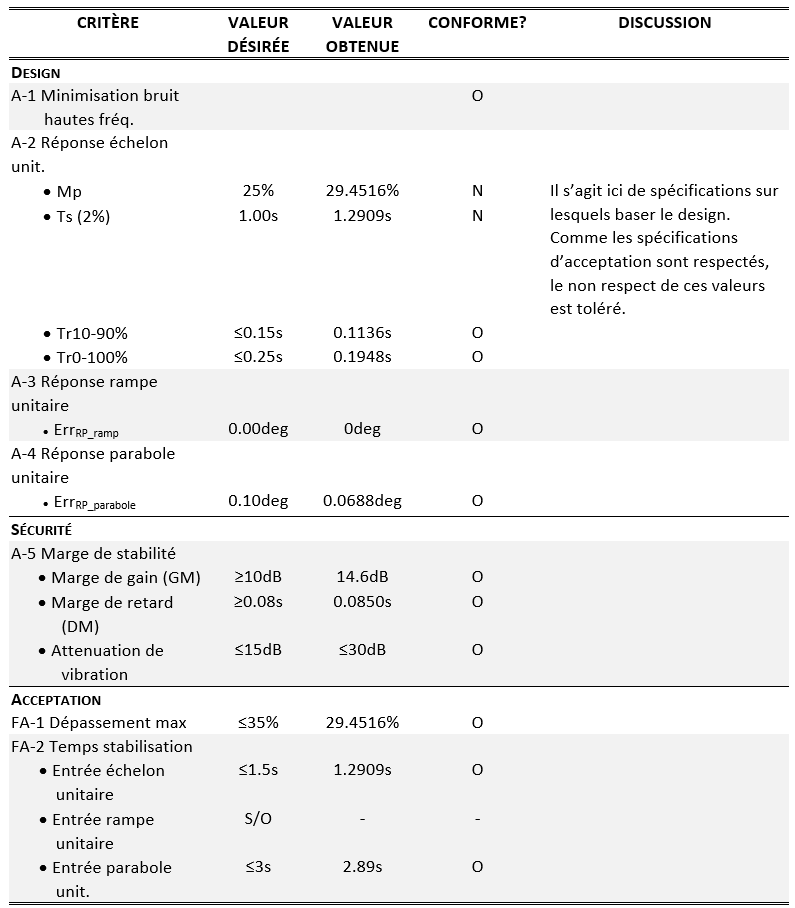
\includegraphics[width=\linewidth]{conformite_A_EL}
\end{center}
Le tableau \ref{tab:conformite_A_EL} présentes les différents critères du clients et les caractéristiques rencontrés par le système de compensation développé plus haut. La majorité des spécificaitons sont rencontrées.\\
La minimisation de l'amplification des hautes fréquences est évaluer de manière qualitative à l'aide de la figure \ref{fig:HF_minimal_EL}. Comme il est possible de le voir, il n'y a que très peu de gain appliqué entre la finale et l'originale dans les hautes fréquence. Deplus, l'orde du gain de cette zone est plus petit que -100 dB, il est donc possible de considérer que les hautes fréquences (le bruit) a été augmenté de manière minimale. Sur l'agrandissement \ref{fig:HF_minimal_EL_zoom} il est mis en évidence que le gain des vibrations est inférieure à -15dB.

%%%%%%% FIGURE %%%%%%%
%double figure
\makebox[\textwidth][c]{
\noindent\begin{minipage}{1.3\textwidth}
 
\begin{minipage}{0.5\textwidth}
\insertFigure{double}{HF_minimal_EL}{1}{Comparaison des lieux de bode}
\end{minipage}%
\begin{minipage}{0.5\textwidth}
\insertFigure{double}{HF_minimal_EL_zoom}{1}{Agrandissement sur les vibrations}
\end{minipage} 

\label{fig:bode_EL} 
\end{minipage}
}
%%%%%%%%%%%%%%%%%%%%%%

La différence de réponse à la parabole unitaire et la parabole permet de confirmer le temps de stabilisation. Il est illustrer à la figure \ref{fig:ramp_EL_A} ce qui confirme l'atteinte de la spécification associée.
%%%%%%% FIGURE %%%%%%%
\insertFigure{simple}{ramp_EL_A}{0.7}{Différence de réponse à la parabole unitaire et la parabole}
%%%%%%%%%%%%%%%%%%%%%%


\subsubsection{Validation de la trajectoire de référence}
Comme pour l'azimut, la trajectoire est très semblables à la consigne mise à part quelque \textit{overshoot} et renflement qui pouvaient être attendu, car  le système final comporte des erreurs en régime permanent et en régime transitoire. Les résultats obtenus sont tout de même acceptable vue que l'allure générale de la courbe n'est que peut différente de la consigne. Le coéfficient de corrélation confirme aussi ce analyse visuel, il est de 0.9994, soit très près de la perfection.
%%%%%%% FIGURE %%%%%%%
\insertFigure{simple}{Verif_trajectoire_A_EL}{0.7}{Validation de la trajectoire de référence}
%%%%%%%%%%%%%%%%%%%%%%
%----------------------------------------------------------------------------------------------------------------------%
\section{Design du télescope B}
\subsection{Azimut}
\subsubsection{Design initial}
\subsubsection{Iterations}

\subsubsection{Conformité}
\subsubsection{Validation de la trajectoire de référence}
\subsection{Élévation}
\subsubsection{Design initial}
\subsubsection{Iterations}

\subsubsection{Conformité}
\subsubsection{Validation de la trajectoire de référence}
%----------------------------------------------------------------------------------------------------------------------%
\section{Conclusion}






\begin{comment}

\section{Filtres FIR}
\noindent\begin{minipage}{\textwidth} 
\begin{minipage}{0.5\textwidth}
  \centering
  \includegraphics[width=.75\linewidth]{ampFIR}
  \captionof{subfigure}{Amplitude}
  \label{FIR:ampFIR}
\end{minipage}%
\begin{minipage}{0.5\textwidth}
  \centering 
  \includegraphics[width=.75\linewidth]{phaseCute} 
  \captionof{subfigure}{Phase} 
  \label{FIR:phaseFIR} 
\end{minipage} 
\captionof{figure}{Filtre IIR} 
\label{FIR} 
\end{minipage}
\end{comment}

\end{document}













